\documentclass[12pt]{beamer}
\usepackage[utf8]{inputenc}
\usepackage[portuguese]{babel}
\usepackage{graphicx}
\usepackage{colortbl}
\usepackage{color}
\usepackage{breqn}
\usepackage{listings}
\usepackage{hyperref}
\usepackage{beamerthemeshadow}

\graphicspath{{./images/} {../diagrams/} {../doc/images}}
\setbeamertemplate{caption}[numbered]

\definecolor{dkgreen}{rgb}{0,0.6,0}
\definecolor{gray}{rgb}{0.5,0.5,0.5}
\definecolor{mauve}{rgb}{0.58,0,0.82}
\definecolor{laranja_claro}{rgb}{1,0.9,0.5}
\definecolor{laranja_escuro}{rgb}{1,0.5,0.2}
\definecolor{azul_claro}{rgb}{0.5,0.9,1}

\lstset{frame=tb,
    language=C,
    frame=tb,
    aboveskip=3mm,
    belowskip=3mm,
    showstringspaces=false,
    columns=flexible,
    basicstyle={\small\ttfamily},
    numbers=left,
    numberstyle=\tiny\color{gray},
    keywordstyle=\color{blue},
    commentstyle=\color{dkgreen},
    stringstyle=\color{mauve},
    breaklines=true,
    breakatwhitespace=true,
    xleftmargin=.05\textwidth,
    xrightmargin=.05\textwidth,
    tabsize=4,
}

\definecolor{azul}{rgb}{0,0,.5}
\setbeamertemplate{navigation symbols}{}

\usetheme{Frankfurt}
\usecolortheme[named=azul]{structure}

\addtobeamertemplate{navigation symbols}{}{%
    \usebeamerfont{footline}%
    \usebeamercolor[black]{footline}%
    \hspace{1em}%
    Página~\insertframenumber~de~\inserttotalframenumber
}

%% Definindo o Autor e o título
\newcommand{\prof}{Renato Bobsin Machado}
\newcommand{\materia}{Redes de Computadores}

\author[Grupo: MQTT]{Larissa L. Wong \and Marco A. G. Pedroso \and Victor E. Almeida}

\title{Protocolo MQTT para sistemas de IoT}
\subtitle{Um estudo técnico/prático}
\date{\today}
\institute{UNIOESTE}
\logo{
\includegraphics[height=1cm]{logo_unioeste.jpg}}

\begin{document}
\frame{\titlepage}

\section{Introdução}\label{Introdução}

\begin{frame}
\frametitle{Conteúdo}
\tableofcontents
\end{frame}

\begin{frame}
    \frametitle{Colocar mais algo para introduzir}
    TODO
\end{frame}

\section{História}\label{História}
\begin{frame}
    \frametitle{Criação do Protocolo}
    Começou a ser projetado durante a década de 1990 por:
    \begin{columns}[c]
        \begin{column}{.5\textwidth}
            \begin{figure}[!htb]
                \centering
                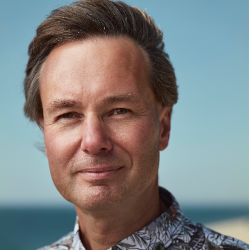
\includegraphics[width=.75\textwidth]{andy_stanford_clark1}
                \caption{\label{fig:andy}Andy Stanford-Clark da IBM}
            \end{figure}
        \end{column}
        \begin{column}{.5\textwidth}
            \begin{figure}[!htb]
                \centering
                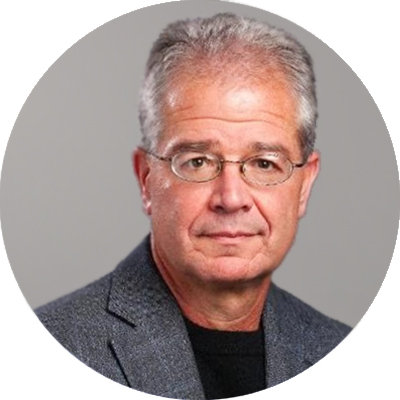
\includegraphics[width=.77\textwidth]{arlen_nipper1}
                \caption{\label{fig:arlen}Arlen Nipper da Cirrus Link/Eurotech}
            \end{figure}
        \end{column}
    \end{columns}
\end{frame}

\begin{frame}
    \frametitle{Problemas a serem resolvidos}
    \begin{itemize}
        \item Resolver o problema de conexão de oleodutos via satélite.
        \item Limitações:
            \begin{itemize}
                \item Alta latência;
                \item Baixa largura de banda;
                \item Dispositivos com pouca bateria.
            \end{itemize}
    \end{itemize}
        
\end{frame}

\begin{frame}
    \frametitle{Requisitos do Protocolo}
    \begin{itemize}
        \item Implementação simples;
        \item Uso de QoS, \textit{Quality of Service} por quem publica a mensagem;
        \item Uso eficiente de largura de banda, baixo \textit{overhead};
        \item Baixo custo energético para envio;
        \item Possibilidade de enviar qualquer tipo de dado;
        \item Possibilidade de manter conexões ativas, prontas para enviar e receber dados;
    \end{itemize}
\end{frame}

\begin{frame}
    \frametitle{Fase do protocolo proprietário}
    \begin{figure}[!htb]
        \centering
        
\includegraphics[width=\textwidth]{logo_mqtt}
        %\caption{\label{fig:logo_mqtt}Logo do MQTT}
    \end{figure}
    \begin{itemize}
        \item Primeira versão implementada no ano de 1999;
        \item Batizado MQTT, \textit{MQ Telemetry Transport}, em referência ao produto da IBM MQ Series
        \item Muito utilizado embarcado em produtos da IBM.
    \end{itemize}
\end{frame}

\begin{frame}[allowframebreaks]
    \frametitle{Fase do protocolo aberto}
    \begin{itemize}
        \item Demanda/Aplicabilidade IoT;
        \item Em 2010 o protocolo se tornou livre;
        \item Primeira versão lançada 3.1;
        \item Investimentos da IBM através da Eclipse Foundation para criar um ecossistema em torno do protocolo.
    \end{itemize}
    \begin{figure}[!htb]
        \centering
        
\includegraphics[width=.5\textwidth]{eclipse_logo}
        %\caption{\label{fig:eclipse_logo}Logo da Eclipse Foundation}
    \end{figure}
    \framebreak
    \begin{figure}[!htb]
        \begin{columns}[c]
            \begin{column}{.5\textwidth}
                
\includegraphics[width=.9\textwidth]{paho_logo}
            \end{column}
            \begin{column}{.5\textwidth}
                
\includegraphics[width=.9\textwidth]{Mosquitto_logo}
            \end{column}
        \end{columns}
        \caption{\label{fig:logos_ferramentas_mqtt}Exemplos de aplicações do ecossistema MQTT}
    \end{figure}
    \framebreak
    \begin{itemize}
        \item No ano de 2013 a IBM buscou padronização com a OASIS;
        \item 29 de outubro de 2014 o MQTT foi aprovado como padrão pela OASIS na sua versão 3.1.1
    \end{itemize}
    \begin{figure}[!htb]
        \centering
        
\includegraphics[width=.8\textwidth]{Oasis_logo}
        %\caption{\label{fig:Oasis_logo}}
    \end{figure}
\end{frame}

\begin{frame}
    \frametitle{Fase atual do protocolo}
    \begin{itemize}
        \item A última versão 5.0 março de 2019;
        \item Funcionalidades modernas como:
            \begin{itemize}
                \item facilidade de conexão e interação com a nuvem;
                \item Tratamento de erros;
            \end{itemize}
        \item Implementações de clientes para diversos sistemas e linguagens;
        \item Implementação de diversos brokers;
        \item Utilizado por grandes empresas tanto software aberto quanto proprietário.
    \end{itemize}
\end{frame}

\section{Prática}\label{Prática}
\begin{frame}
    \frametitle{Dispositivos e softwares da parte prática}
    \begin{itemize}
        \item Esp32:
            \begin{itemize}
                \item Sensor Adafruit BMP-280;
                \item Relay para ligar lâmpada;
                \item C/C++ (Framework Arduino e ESP-IDF);
            \end{itemize}
        \item Raspberry:
            \begin{itemize}
                \item Docker executando o broker mosquitto;
                \item Cliente inscrito no tópico ``\#''
            \end{itemize}
    \end{itemize}
\end{frame}

\begin{frame}
    \frametitle{Diagrama da aplicação}
    \begin{figure}[!htb]
        \centering
        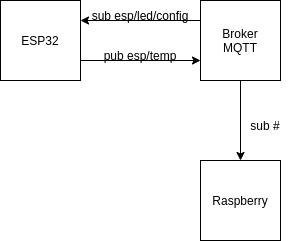
\includegraphics[width=.7\textwidth]{aplication}
        \caption{\label{fig:aplication} Dispositivos e tópicos utilizados}
    \end{figure}
\end{frame}
\begin{frame}
    \frametitle{Mão na massa!!}
    \begin{figure}
        \centering
        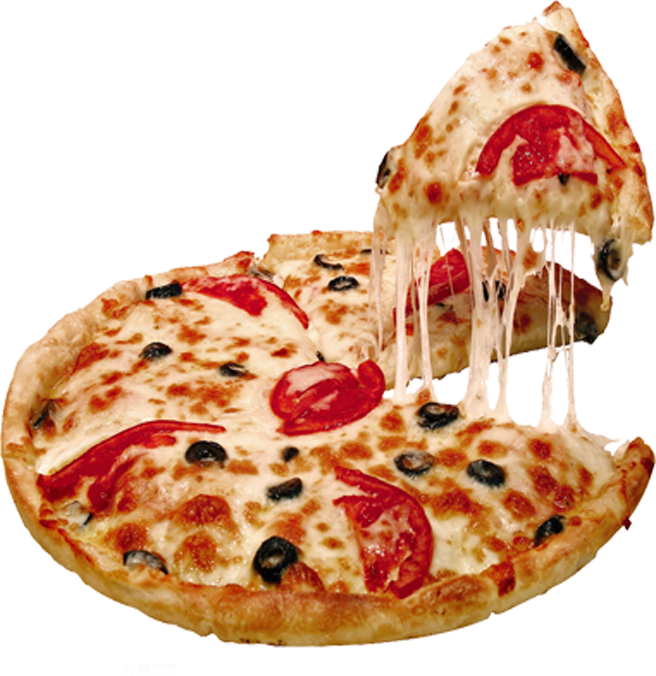
\includegraphics[width=.3\textwidth]{pizza.png}
        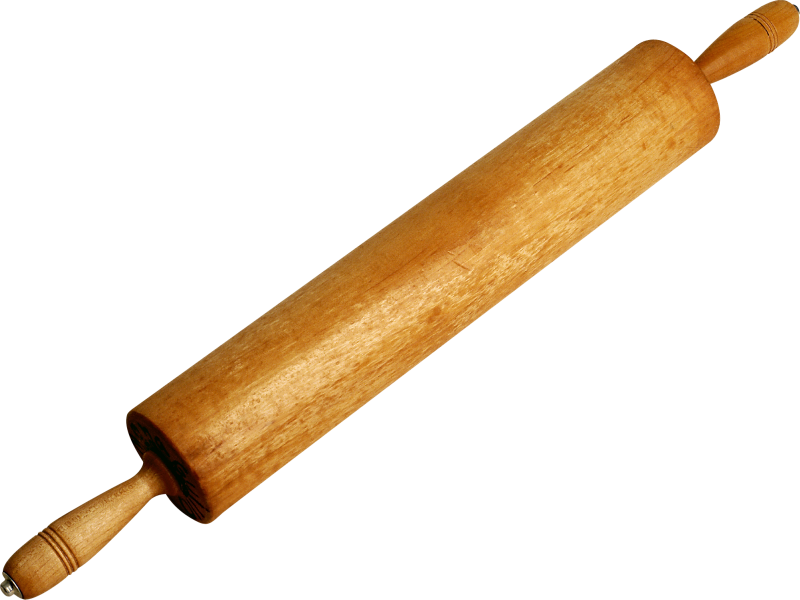
\includegraphics[width=.3\textwidth]{rolo.png}
        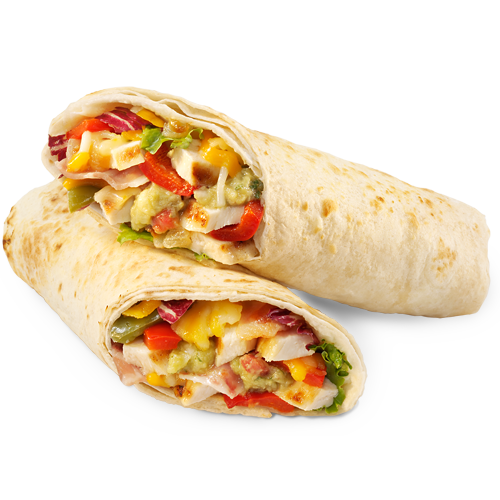
\includegraphics[width=.3\textwidth]{burrito.png}
    \end{figure}
\end{frame}

\section{Conclusão}
\begin{frame}
    \frametitle{Agradecimentos}
    \centering
    \Huge{Perguntas?}
    \begin{figure}
        \centering
        
\includegraphics[width=.3\textwidth]{alerta.png}
        
\includegraphics[width=.3\textwidth]{perigo.png}
        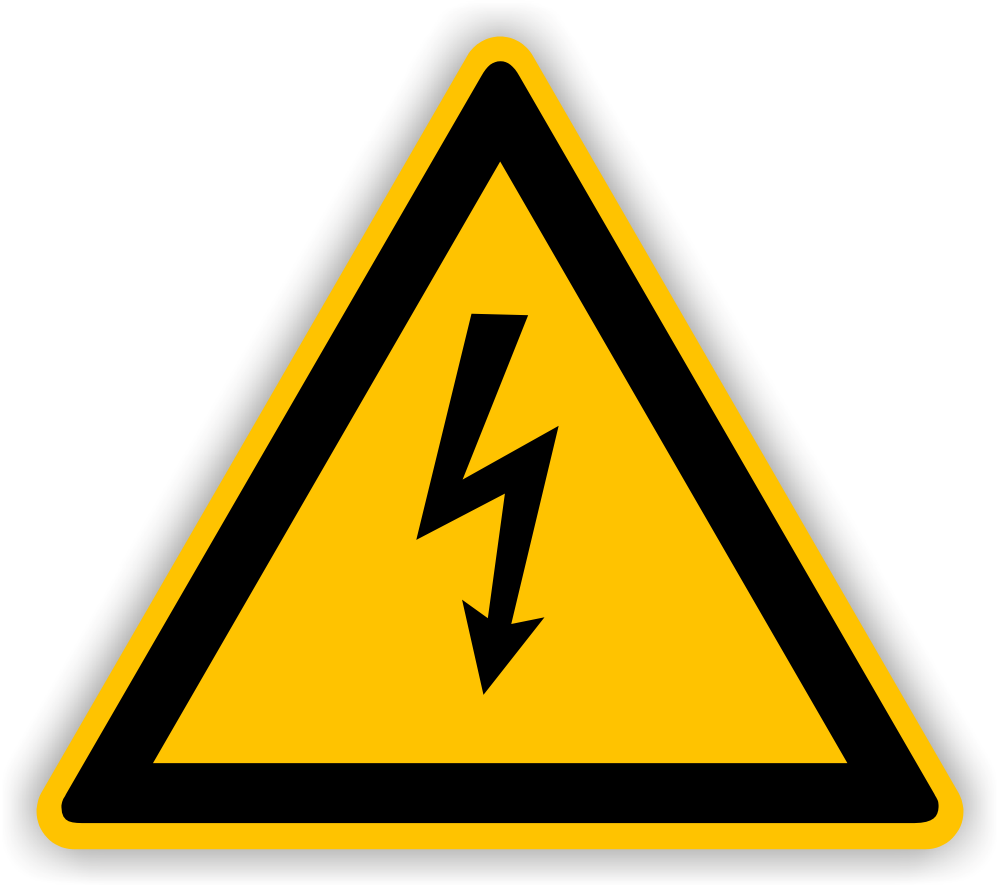
\includegraphics[width=.3\textwidth]{eletricidade.png}
    \end{figure}
    \Huge{Obrigado pela atenção}
\end{frame}

\end{document}
